%%%%%%%%%%%%%%%%%%%%%%%%%%%%%%%%%%%%%%%%%
% Thin Sectioned Essay
% LaTeX Template
% Version 1.0 (3/8/13)
%
% This template has been downloaded from:
% http://www.LaTeXTemplates.com
%
% Original Author:
% Nicolas Diaz (nsdiaz@uc.cl) with extensive modifications by:
% Vel (vel@latextemplates.com)
%
% License:
% CC BY-NC-SA 3.0 (http://creativecommons.org/licenses/by-nc-sa/3.0/)
%
%%%%%%%%%%%%%%%%%%%%%%%%%%%%%%%%%%%%%%%%%

%----------------------------------------------------------------------------------------
%	PACKAGES AND OTHER DOCUMENT CONFIGURATIONS
%----------------------------------------------------------------------------------------

\documentclass[11pt]{article} % Font size (can be 10pt, 11pt or 12pt) and paper size (remove a4paper for US letter paper)

\usepackage{graphicx} % Required for including pictures
\usepackage{epstopdf}
\usepackage{wrapfig} % Allows in-line images
\usepackage{fullpage}
\usepackage{hyperref} % hyper reference
\usepackage{seqsplit}

\usepackage[protrusion=true,expansion=true]{microtype} % Better typography. Comment this line if want to use XeTex.
\usepackage{mathpazo} % Use the Palatino font. Comment this line if want to use XeTex.
\usepackage[T1]{fontenc} % Required for accented characters. Comment this line if want to use XeTex.
%\usepackage{fontspec} % For loading fonts
%\setmainfont{Minion Pro} % Main document font
%\usepackage{xltxtra}
\linespread{1.05} % Change line spacing here, Palatino benefits from a slight increase by default

\makeatletter
\renewcommand\@biblabel[1]{\textbf{#1.}} % Change the square brackets for each bibliography item from '[1]' to '1.'
\renewcommand{\@listI}{\itemsep=0pt} % Reduce the space between items in the itemize and enumerate environments and the bibliography

\renewcommand{\maketitle}{ % Customize the title - do not edit title and author name here, see the TITLE block below
\begin{flushright} % Right align
{\LARGE\@title} % Increase the font size of the title

\vspace{50pt} % Some vertical space between the title and author name

{\large\@author} % Author name
\\\@date % Date

\vspace{40pt} % Some vertical space between the author block and abstract
\end{flushright}
}

%----------------------------------------------------------------------------------------
%	TITLE
%----------------------------------------------------------------------------------------

\title{\textbf{Detectors and Methods for QGP Measurements}}

\author{\textsc{Shih-Kai Lin} % Author
\\{\textit{University of Houston}}} % Institution

\date{Fall 2013} % Date

%----------------------------------------------------------------------------------------

\begin{document}

\maketitle % Print the title section

%----------------------------------------------------------------------------------------
%	ABSTRACT AND KEYWORDS
%----------------------------------------------------------------------------------------

%\renewcommand{\abstractname}{Summary} % Uncomment to change the name of the abstract to something else

\begin{abstract}
First I will talk about a brief derivation of the Bethe formula, which is one of the most important formula in particle detection. Then how momentum is measured in accelerator experiments is discussed. Then I move on to particle identification. After all these somewhat mundane topics in textbooks, centrality and temperature measurements are discussed which are more specific to heavy ion experiments.
\end{abstract}

%\hspace*{3,6mm}\textit{Keywords:} lorem , ipsum , dolor , sit amet , lectus % Keywords

\vspace{30pt} % Some vertical space between the abstract and first section

%----------------------------------------------------------------------------------------
%	ESSAY BODY
%----------------------------------------------------------------------------------------

\section{Ionization Energy Loss}

Particles are detected through interactions with matter. Among the energy loss mechanisms, the ionization energy loss is of primary importance. Even for neutral particles, they are very likely to be detected by their decaying to or interactions producing charged particles. Here I would like to go through the derivation of Bethe's equation with only knowledge acquired in the graduate level courses. Among the literature, I found J.D. Jackson's treatment \cite{jackson98} particularly enlightening. I will follow his text and fill the missing steps.

To start with, note that the ionization energy loss is due to the single collision with the atomic or molecular electrons. Since the electron binding energy is negligible compared to the energy of the incident particle, we can regard the process as a fixed target collision, with the electron being the stationary target. Suppose the mass of the incident particle is much larger than the mass of the electron, we can view the process in the rest frame of the incident particle and approximate the incident particle as a fixed charge center. Suppose in the lab frame an incident particle with charge $ze$, mass $M$ and speed $\beta c$ collides with an electron with charge $-e$ and mass $m$. In the rest frame of the incident particle we can apply the Rutherford differential scattering cross-section formula, which is
\begin{equation}
\frac{d\sigma}{d\Omega}=\left( \frac{ze^2}{2pv} \right)^2 \frac{1}{\sin^4\frac{\theta}{2}}
\end{equation}
where $p=\gamma m\beta c$, $v=\beta c$ and $\theta$ are the momentum, speed and scattering angle of the electron in the rest frame of the incident particle, respectively.

Since we do experiments in the lab frame, we have to make transformations of the quantities to the lab frame. The idea here is to cast the variables in equation (1) into some Lorentz invariant variables and reexpress the variables with the lab frame quantities. The Lorentz scalar used here is the minus 4-momentum transfer squared,
\begin{equation}
Q^2\equiv-(\underline{p}-\underline{p}')^2=(\vec{p}-\vec{p}')^2=4p^2\sin^2\frac{\theta}{2}
\end{equation}
since energy is conserved in this process and $|\vec{p}|=|\vec{p}'|=p$. In terms of $Q^2$ variable, the cross section is
\begin{eqnarray}
\frac{d\sigma}{dQ^2} &=& \frac{d\sigma}{d\Omega}\frac{d\Omega}{dQ^2} = \frac{d\sigma}{d\Omega}\frac{2\pi\sin\theta d\theta}{dQ^2}\nonumber \\
&=& \left[\left( \frac{ze^2}{2pv} \right)^2 \frac{1}{\sin^4\frac{\theta}{2}}\right] (2\pi\sin\theta)\left( \frac{1}{2p^2\sin\theta} \right) \nonumber \\
&=& 4\pi\left( \frac{ze^2}{\beta cQ^2} \right)^2
\end{eqnarray}

Since $\beta$ is the relative speed of the two particles which has the same value in each rest frame of the two particles, if we can express $Q^2$ in the lab frame, we have the cross section formula in the lab frame. The 4-momenta of the electron in the lab frame before and after the collision are $(mc,0)$ and $(\sqrt{p^2+m^2c^2},\vec{p})$, therefore the $Q^2$ is
\begin{equation}
Q^2=p^2-\left( \sqrt{p^2+m^2c^2}-mc \right)^2=2m\sqrt{p^2+m^2c^2}-2m^2=2mT
\end{equation}
where $T$ is the kinetic energy of the electron acquired in the collision, which is exactly the energy loss by the incident particle in the lab frame. The differential cross section per unit energy loss in the lab frame becomes
\begin{equation}
\frac{d\sigma}{dT}=2m\cdot 4\pi\frac{z^2e^4}{c^2\beta^2\cdot 4m^2T^2}=\frac{2\pi z^2e^4}{mc^2\beta^2T^2}
\end{equation}

Suppose the matter the incident particle goes through has an atomic number density $N$ per unit volume and each atom has $Z$ electrons. The interaction probability per unit length of losing energy $T$ is $NZ\frac{d\sigma}{dT}dT$, so the mean energy loss per unit length is
\begin{equation}
-\frac{dE}{dx}=\int_I^{T_{max}}NZT\frac{d\sigma}{dT}dT=\frac{2\pi NZz^2e^4}{mc^2\beta^2}\ln\left( \frac{T_{max}}{I} \right)
\end{equation}
where $I$ is the mean excitation energy and $T_{max}$ is the maximum energy transfer. To obtain $T_{max}$, let's go back to the incident particle's rest frame. The maximum energy transfer then corresponds to the backward scattering. If the incident particle travels in the $+z$ direction in the lab frame, after direction reversal the electron will have 4-momentum $(\gamma mc,0,0,\gamma\beta mc)$ in the rest frame of the incident particle. Making a boost in the $-z'$ direction, we have
\begin{equation}
T_{max}=E-mc^2=c\gamma(\gamma mc+\gamma\beta^2mc)-mc^2 = 2\gamma^2\beta^2mc^2
\end{equation}
Substitute $T_{max}$ into equation (6) we have
\begin{equation}
-\frac{dE}{dx}=\frac{2\pi NZz^2e^4}{mc^2\beta^2}\ln\left( \frac{2\gamma^2\beta^2mc^2}{I} \right)
\end{equation}
This is the formula commonly seen in the enthusiastic derivation.

A more exact form would be
\begin{equation}
-\frac{dE}{dx}=\frac{2\pi NZz^2e^4}{mc^2\beta^2}\left( \ln\left( \frac{2\gamma^2\beta^2mc^2}{I} \right) -\beta^2\right)
\end{equation}
The origin of the additional $-\beta^2$ term is rooted in the more exact treatment of the differential scattering cross section, namely, Mott scattering. The Mott scattering cross section assumes the form
\begin{equation}
\left( \frac{d\sigma}{dT} \right)_{Mott}=\left( \frac{d\sigma}{dT} \right)_{Rutherford}\left( 1-\beta^2\sin^2\frac{\theta}{2} \right)
\end{equation}
, where the additional term is due to the electron spin effect.

From equations (2), (4) and (7) we have $\sin^2\frac{\theta}{2}=\frac{T}{T_{max}}$. Therefore, in equation (6) if we use the Mott scattering cross section instead of the Rutherford's, we arrive at the more exact form (9). Of course this is still not the final equation cited in the PDG. The even better energy loss formula is
\begin{equation}
-\frac{dE}{dx}=\frac{2\pi NZz^2e^4}{mc^2\beta^2}\left( \ln\left( \frac{2\gamma^2\beta^2mc^2}{I} \right) -\beta^2-\frac{\delta}{2}\right)
\end{equation}
in which a density-effect correction of the matter $\delta$ is included. In gas detectors this term is negligible.

%------------------------------------------------

\section{Measurement of Momentum}

We study elementary particles physics through measuring the particles' momentum and energy. Once momentum is determined, further determination of the particle velocity makes particle identification possible.

The rate of change of momentum and energy of a charged particle with charge $q$ and velocity $\vec{v}$ in an external magnetic field $\vec{B}$ can be written, owning to Lorentz force law and the fact that magnetic force does no work, as
\begin{eqnarray}
\frac{d\vec{p}}{dt}&=&q\vec{v}\times\vec{B}=\frac{q}{\gamma m}\vec{p}\times\vec{B} \label{eq:lozfl} \\
\frac{dE}{dt}&=&0
\end{eqnarray}
Since the energy is constant in time, so is the speed of the particle therefore also $\gamma$. Solution to eq. (\ref{eq:lozfl}) is a helix with gyration radius $a$. Denoting the momentum perpendicular to the magnetic field $\vec{p}_\perp$, it satisfies the equation
\begin{equation}
cp_\perp=qBa
\end{equation}
Therefore if we can make space-time snapshots along the particle's track, we can reconstruct the track and then obtain the momentum.

%------------------------------------------------

\section{Charged Particle Identification}

Decayed particles have to be identified in order to study parent particles with short lifetime. Here I expand on the ionization loss methods for charged particle identification talked about in the lecture.

\subsection{Identification by Ionization Losses}

Let's take a closer look at the Bethe formula, equation (9). When the particle momentum is small, we can make a Taylor series expansion on the $ln$ term and keep only the lowest order term. Then $\frac{dE}{dx}\sim \frac{1}{\beta^2} \sim \frac{1}{p^2}$. This reflects on the fast drop of the curve in the small momentum region. Since $p=\gamma\beta mc$, we can substitute the $\beta$'s and $\gamma$'s in Bethe formula with $p$,
\begin{equation}
-\frac{dE}{dx}=\frac{2\pi NZz^2e^4}{mc^2}\left[ \left( \frac{p^2+M^2c^2}{p^2} \right)  \ln\left( \frac{2p^2m}{IM^2} \right) -1 \right]
\end{equation}
If Argon parameters at STP and particle masses for muon, pion, kaon, proton and D meson are used in the formula, the energy losses as a function of momentum is shown in Figure \ref{fig:dEdxcurve}, which mirrors the PEP-4 results, Figure \ref{fig:dEdxpep4} quit well. The difference in the absolute value would be attributed to the different pressure and gas composition PEP-4 used (80\% argon and 20\% methane gas at 8.5 atmosphere).

\begin{figure}
    \centering
    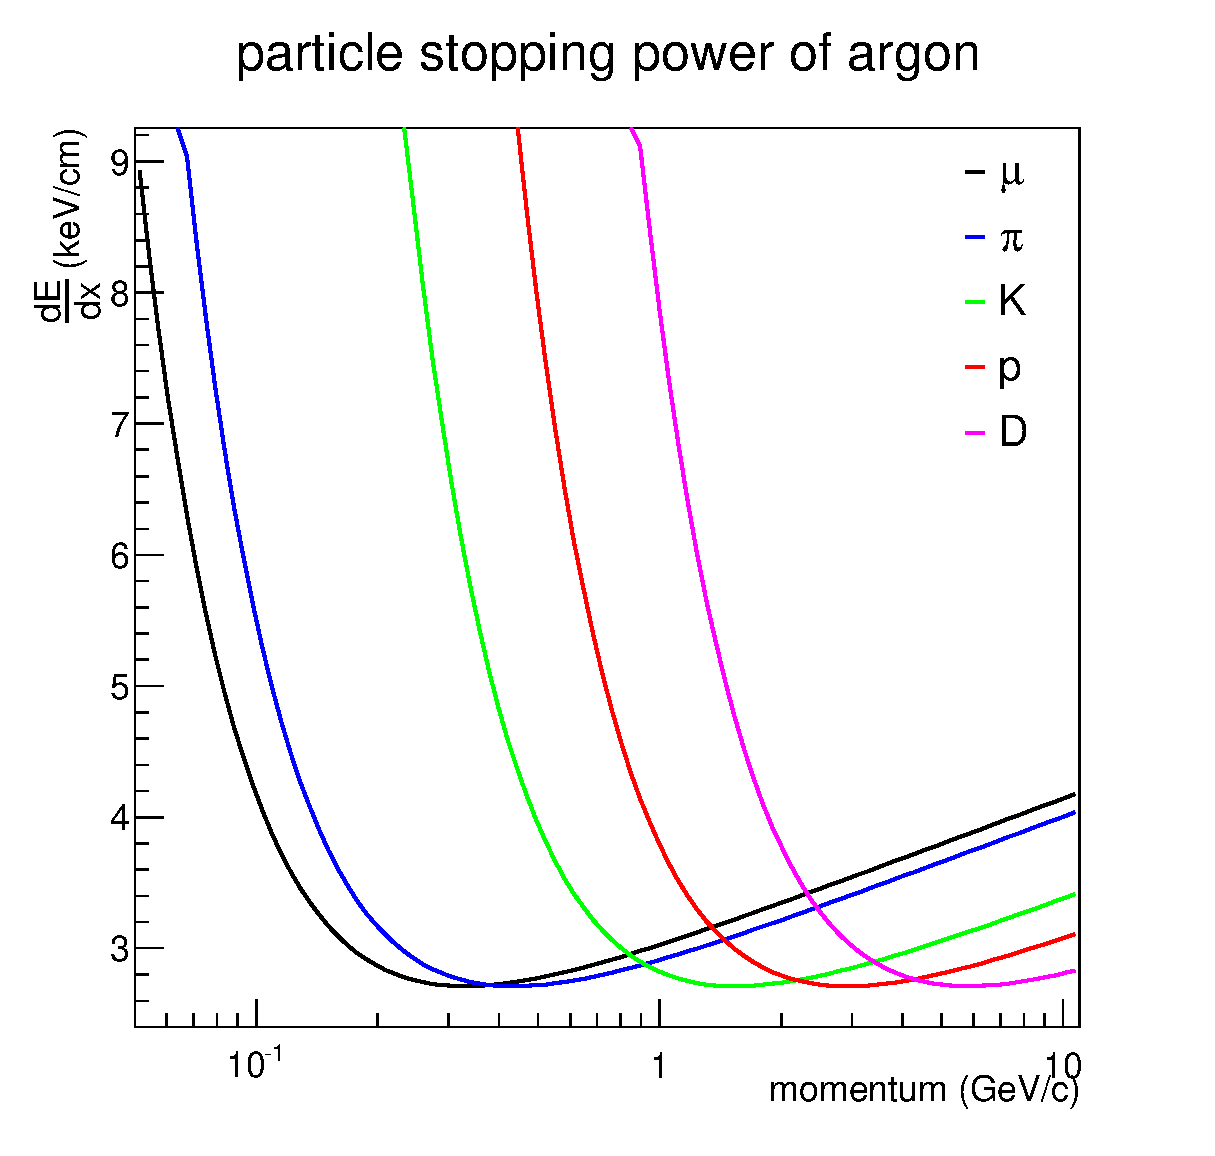
\includegraphics[width=0.6\textwidth]{plots/dEdx.eps}
    \caption{particle stopping power of Argon at STP}
    \label{fig:dEdxcurve}
\end{figure}

\begin{figure}
    \centering
    \includegraphics[width=0.6\textwidth]{plots/pep_pid.png}
    \caption{PEP-4 ionization energy loss}
    \label{fig:dEdxpep4}
\end{figure}

\begin{figure}
    \centering
    \includegraphics[width=0.6\textwidth]{plots/ALICE_TPC.pdf}
    \caption{3D view of the ALICE TPC field cage}
    \label{fig:alicetpc}
\end{figure}

In collider experiments the ionization energy loss is usually measured by Time Projection Chambers (TPCs). Figure \ref{fig:alicetpc} shows the ALICE TPC. It is just a huge cylindrical gas counter with multiwire proportional chambers mounted on the two ends. The cylindrical body is divided into two drift regions by the central high voltage electrode which is operated at 100 kV which provides a precise axial electric field of 400 V/cm. When a charged particle passes through the chamber, it ionises the $Ne$ atoms along the way. The ionised electrons are then guided by the electric field and drift to the MWPCs for readout. In the meanwhile the arrival time is also available, therefore a complete 3D particle track can be reconstructed. Through the relation
\begin{equation}
x\left\langle\frac{dE}{dx}\right\rangle=\langle N_I\rangle W
\end{equation}
where $x$ is the length the particle traverses, $\langle N_I\rangle$ the measured number of ionised electrons and $W$ the average energy spent for the creation of one electron/ion pair, we can obtain $dE/dx$.


%------------------------------------------------

\section{Centrality Measurement}

Centrality is an important parameter in heavy ion experiments since it is a fundamental characterization of a collision event and lots of heavy ion experiment results are presented as functions of centrality. The roadmap of measuring centrality can be depicted in the following procedure:
\begin{equation}
\underbrace{\frac{dN_{ch}}{d\eta}}_{experimental \: observable} \propto \overbrace{\left( N_{coll}, N_{part} \right)}^{modeled\:by\:Glauber} \propto \underbrace{b}_{known\:in\:simulations}\rightarrow centrality
\end{equation}

The Glauber model \cite{miller07} was developed by the Nobel Laureate Roy Glauber in the $1950$s to address the problem of high energy collisions with composite particles. This model later on is found useful in calculating the total cross sections of proton nucleus and ion nucleus scattering. Nowadays the Glauber Monte Carlo Models are used in determining the centrality of the heavy ion collisions.

There are two routes to the $N_{coll}$ and ${N_{part}}$ with the Glauber Model. One is to use the full analytical theory which involves a $2(A+B+1)$ dimensional integral over the impact parameter and each of the nucleon position. For Au+Au collision it is more than 800 dimensional and renders the problem almost unsolvable. The other way is to use Monte Carlo simulation. With the aid of computers, we can simply model the nucleus as uncorrelated nucleons sampled from measured density distributions. Then two nuclei are projected to each other with a known impact parameter $b$ and with the knowledge of the measured nucleon-nucleon inelastic scattering cross section, the interaction probability between two nucleons can be calculated in accordance with the distance between their centroids.

Bellow steps of Glauber Monte Carlo Model are summarized.
\begin{enumerate}
\item Create Nuclei
  \begin{enumerate}
    \item The size and shape of nuclei are determined by electron scattering.
    \item For each nucleon a random position is drawn from the three-parameter Woods-Saxon charge distribution of the form,
      \begin{equation}
      \rho(r,\theta)=\left\{
        \begin{array}{lr}
        \rho_0 \left( \frac{1+w\left(\frac{r}{c}\right)^2}{1+e^x} \right) & \textit{if} \; r<c \\
        \rho_0 \left( \frac{1+w}{1+e^x} \right) & \textit{if} \; r \ge c
        \end{array}
        \right.
      \end{equation}
      \begin{equation}
      \textit{where}\; x=\frac{r-c(1+\beta_{20}Y_{20}(\theta)+\beta_{40}Y_{40}(\theta))}{a(1+\beta_{20}Y_{20}(\theta)+\beta_{40}Y_{40}(\theta))}
      \end{equation}
      The parameters for some relevant nuclei are summarized in the following table \cite{flores12}.
      \begin{center}
      \begin{tabular}{|c|c|c|c|c|c|c|}
      \hline
       & $\rho_0$ & $w$ & $a$ & $c$ & $\beta_{20}$ & $\beta_{40}$ \\
       \hline
       Au & 0.169 & 0 & 0.535 & 6.38 & -0.131 & -0.031 \\
       \hline
       Pb & 0.1600 & 0 & 0.549 & 6.624 & 0 & 0 \\
       \hline
       Cu & 0.1701 & 0 & 0.586 & 4.214 & 0.162 & -0.006 \\
       \hline
       U & 0.127 & 0.5 & 0.5 & 6.8 & 0.254 & 0.052 \\
       \hline
      \end{tabular}
      \end{center}
  \end{enumerate}
\item Define orientations and impact parameter of the nuclei
	\begin{enumerate}
	\item Generate an orientation randomly from a uniform distribution on the unit sphere.
	\item Draw a random impact parameter from the distribution
	\begin{equation}
		\frac{d\sigma}{db}=2\pi b
	\end{equation}
	\item Rotate the whole nucleus and translate it by $b$.
	\end{enumerate}
\item Compute $N_{part}$ and $N_{coll}$ \\
	Define the radius of a nucleon as $r_{nucleon}=\sqrt{\sigma_{NN}/\pi}$
	\begin{enumerate}
	\item if the distance between 2 nucleons $d_{NN}<2r_{nucleon}$, increment $N_{coll}$.
	\item if $N_{coll}>0$, increment $N_{part}$.
	\end{enumerate}
\end{enumerate}


\begin{figure}
    \centering
    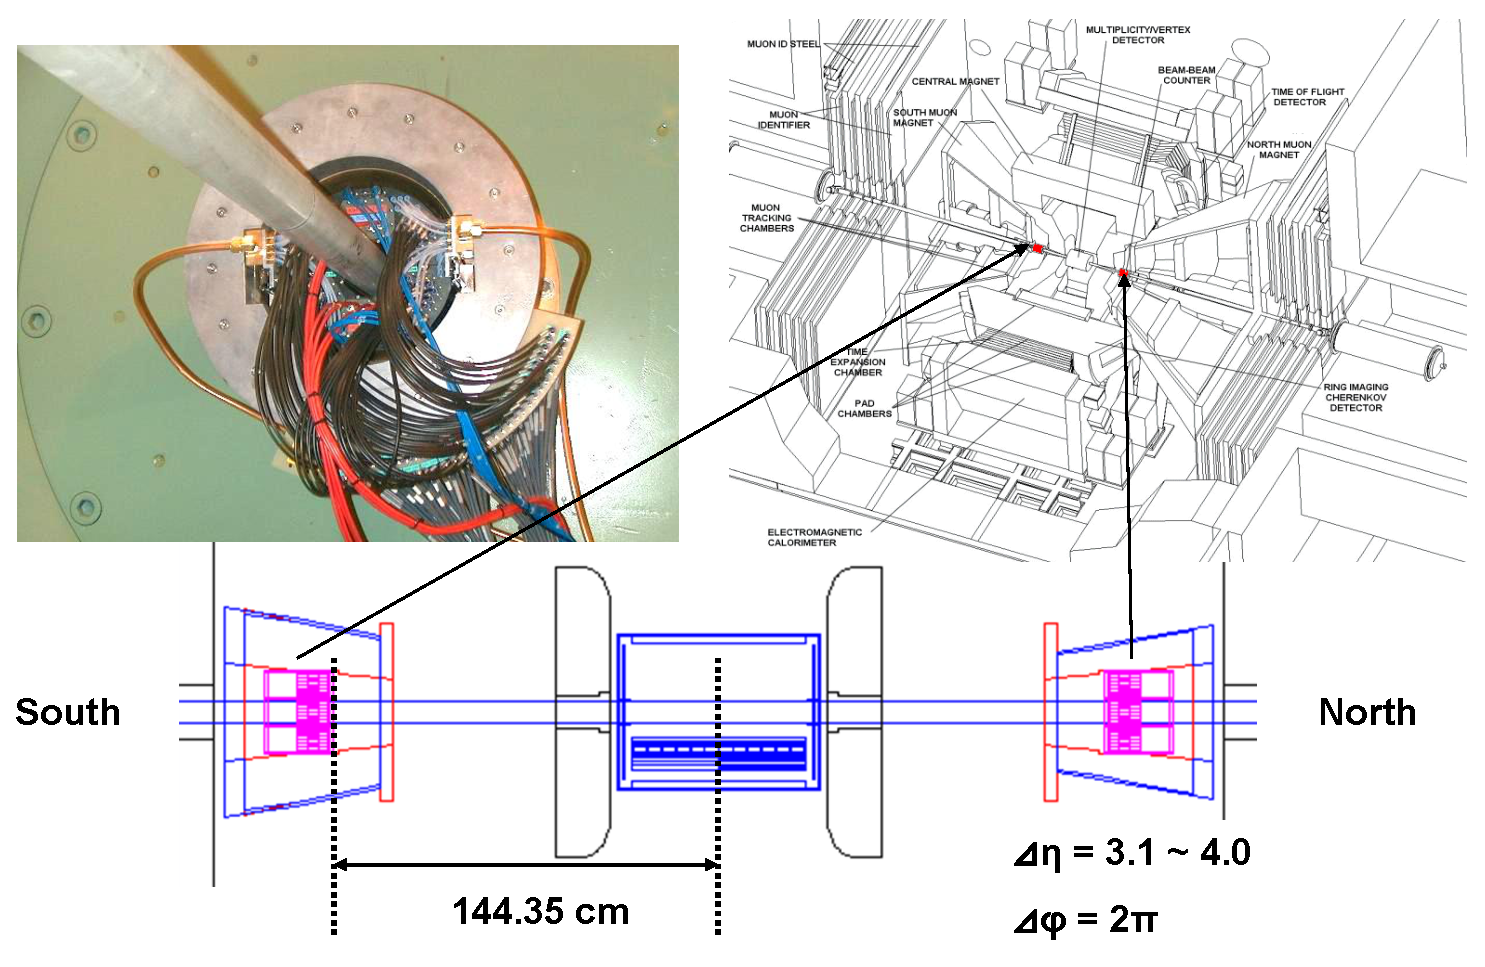
\includegraphics[width=0.6\textwidth]{plots/PHENIX_BBC.eps}
    \caption{PHENIX BBC}
    \label{fig:phenixbbc}
\end{figure}

For different experiments there are different ways to extract centrality from the experimental observables. Here I take PHENIX as an example. Figure \ref{fig:phenixbbc} shows the PHENIX beam beam counter (BBC). The two BBCs each consist of 64 photomultiplier tubes used for detecting Cheremkov light produced by quartz radiators. The purposes of PHENIX BBC include offering minimum bias trigger, offering starting time for time-of-flight measurement, measuring z-vertex and of course, centrality measurement. To make correspondence between the BBC $N_{hit}$ and Glauber Monte Carlo (GMC) $N_{part}$, one first draw the $N_{part}$ spectrum by following the steps mentioned in the previous paragraph as in Figure \ref{fig:npartspec}. Now it is known that for a given $N_{part}$ the BBC $N_{hit}$ spectrum follows negative binomial distribution (NBD),
\begin{equation}
NBD(N_{part},\mu,k)=\frac{\Gamma(N_{part}+k)}{\Gamma(k)N_{part}!}\left( \frac{\mu}{k} \right)^{N_{part}}\frac{1}{(1+\mu/k)^{N_{part}+k}}
\end{equation}
here $\mu=\langle N_{part}\rangle$ and $k$ is related to the width of the distribution. Denote the GMC $N_{part}$ spectrum by $GMC(N_{part})$, the BBC $N_{hit}$ spectrum can be written as
\begin{equation}\label{eq:bbcformula}
BBC(N_{hit})=\epsilon(N_{hit})\sum\limits_{N_{part}}NBD(N_{part},\mu,k)\times GMC(N_{part})
\end{equation}
where $\epsilon(N_{hit})$ is the BBC detection efficiency. By fitting the BBC $N_{hit}$ spectrum to equation (\ref{eq:bbcformula}) one can get $\mu$ and $k$. Once $\mu$ and $k$ are given, one can simple smear each $N_{part}$ with the NBD distribution and find the mean value of the BBC $N_{hit}$ number. Then a lookup table from $N_{hit}$ to $N_{part}$ is thus constructed.

\begin{figure}
    \centering
    \includegraphics[width=0.6\textwidth]{plots/Npart_spec.pdf}
    \caption{$N_{part}$ spectrum from GMC}
    \label{fig:npartspec}
\end{figure}



%------------------------------------------------

\section{Temperature Measurement}

It is rather eye-catching for a layman when he sees the press release saying that the RHIC experiment created matter at a temperature of 4 trillion degrees Celsius, 250,000 times hotter than the core of the Sun. Of course at this high temperature and small scale we cannot just insert a thermometer into the QGP and get the reading from it. How to measure the QGP initial temperature then poses an interesting question.

D. d'Enterria et al. \cite{enterria06}, T. Peitzmann \cite{peitzmann} and A. Adare et al. \cite{adare09} give an overview of getting the initial temperature from $Au+Au$ collisions. The temperature information is actually carried by thermal photons, a kind of direct photons. Direct photons are photons produced directly in the scattering process, not from decays. There are two major categories of direct photons. When $p_T$ is high, the spectrum is dominated by prompt photons produced in hard scattering processes. When $p_T$ is low, the spectrum is dominated by thermal photons from thermal productions. Since photons and leptons interact weakly(electromagnetically) with the medium, by studying photons and leptons we can gain insights into the initial condition of the QGP.

Figure \ref{fig:inv_ph_yield} shows the PHENIX invariant yield of direct photons as a function of $p_T$. The three curves on $p+p$ data are from NLO pQCD calculation, which fit the data quite well. The $p+p$ data can be well described by the modified power law function
\begin{equation}
\frac{A_{pp}}{\left( 1+\frac{p_T}{b} \right)^n}
\end{equation}
where $A_{pp}$ is an overall constant. Now we can scale the $p+p$ data by $T_{AA}$, the nuclear overlap function in Glauber Model. For a given centrality class, $T_{AA}$ can be obtained by the relation \cite{tannenbaum}
\begin{equation}
T_{AA}=\frac{\langle N_{coll} \rangle}{\sigma_{nn}}
\end{equation}
It is evident from the figure that the direct photon yield in the low-$p_T$ range increases faster than the binary-scaled $p+p$ yield. The $Au+Au$ yield now can be fit to an exponential plus the $T_{AA}$ scaled $p+p$ modified power law function
\begin{equation}
Ae^{-\frac{p_T}{T}}+T_{AA}\frac{A_{pp}}{\left( 1+\frac{p_T}{b} \right)^n}
\end{equation}
There are only 2 free parameters here, namely $A$ and $T$. The fitted temperature for central $Au+Au$ collision is $T=221\pm 19^{stat} \pm 19^{syst}$, which is equivalent to 2.4 trillion degrees Celcius.

\begin{figure}
    \centering
    \includegraphics[width=0.5\textwidth]{plots/direct_photon_spectrum.pdf}
    \caption{PHENIX invariant yield of direct photons as a function of $p_T$}
    \label{fig:inv_ph_yield}
\end{figure}

\begin{figure}
    \centering
    \includegraphics[width=0.7\textwidth]{plots/direct_photon_fraction.pdf}
    \caption{The fraction of the direct photon component as a function of $p_T$}
    \label{fig:inv_ph_r}
\end{figure}

To get the direct photon yield could be very challenging. In principle, any source of high-energy direct photons and also emits virtual photons which materialize into dilepton pairs. When the $p_T$ of the $e^+e^-$ pair is much lager than its invariant mass $m_{ee}$, the yield of virtual photons is approximately the same as that of the real photons. Therefore in this region, the yield of real photons can be deduced from measurement of $e^+e^-$ pairs.

Figure \ref{fig:inv_ph_r} shows the fraction of the direct photon to the total photon as a function of $p_T$. The inclusive photon spectra can be obtained by
\begin{equation}
\frac{dN^{incl}_{\gamma}}{dp_T}=\frac{N^{data}_{ee}}{N^{cocktail}_{ee}}\times \frac{dN^{cocktail}_{\gamma}}{dp_T}
\end{equation}
where $N^{data}_{ee}$ is the measured yield of electron pairs for a given $p_T$ bin, $N^{cocktail}_{ee}$ is the yield of the electron pairs in the hadronic cocktail calculation and $\frac{dN^{cocktail}_{\gamma}}{dp_T}$ is the yield of photons in the same calculation. By using the fraction of the direct photon, we can get the direct photon spectra. Then we can cast the spectra into the invariant yield spectra for temperature fitting.


%----------------------------------------------------------------------------------------
%	BIBLIOGRAPHY
%----------------------------------------------------------------------------------------

\bibliographystyle{unsrt}

\bibliography{sample}

\begin{thebibliography}{9}

\bibitem{jackson98}
  Jackson J.D.,
  \emph{Classical Electrodynamics}.
  New York: John Wiley \& Sons.,
  3rd Edition,
  1998.

\bibitem{miller07}
  Michael L. Miller et al.,
  \emph{Glauber Modeling in High-Energy Nuclear Collisions}.
  Annu. Rev. Nucl. Part. Sci. 2007. 57:205-43.

\bibitem{flores12}
  Flores C.,
  \emph{Glauber Modeling in Heavy Ion Collisions}.
  %\seqsplit{http://nuclear.ucdavis.edu/\textasciitilde calderon/Presentations/Phy224C-IntroRHI-Lec7-Glauber\_Talk.pdf}
  \href{http://nuclear.ucdavis.edu/~calderon/Presentations/Phy224C-IntroRHI-Lec7-Glauber_Talk.pdf}{\seqsplit{http://nuclear.ucdavis.edu/\textasciitilde calderon/Presentations/Phy224C-IntroRHI-Lec7-Glauber\_Talk.pdf}}

\bibitem{enterria06}
  D. d'Enterria, D. Peressounko,
  \emph{Probing the QCD equation of state with thermal photons in nucleus-nucleus collisions at RHIC}.
  Eur. Phys. J. C 46, 451-464 (2006).

\bibitem{peitzmann}
  T. Peitzmann,
  \emph{Direct Photon Production in Heavy Ion Reactions}.
	\href{http://agenda.nikhef.nl/getFile.py/access?resId=5&materialId=0&confId=536}{\seqsplit{http://agenda.nikhef.nl/getFile.py/access?resId=5\&materialId=0\&confId=536}}

\bibitem{adare09}
  A. Adare et al.,
  \emph{Detailed measurement of the $e^+e^-$ pair continuum in $p+p$ and $Au+Au$ collisions at $\sqrt{s_{NN}}=200$ GeV and implications for direct photon production}.
	Phys.Rev.C81:034911,2010.

\bibitem{tannenbaum}
	M. J. Tannenbaum,
  \emph{Thickness function and Pointlike Scaling for Hard Scattering}.
	PHENIX analysis note AN057.


\end{thebibliography}
%----------------------------------------------------------------------------------------

\end{document}